\chapter{Исследование существующих алгоритмов построения выпуклых оболочек} \label{chapt1}

\section{Существующие алгоритмы построения выпуклых оболочек} \label{sect1_1}

За долгое время развития вычислительной геометрии появилось огромное количество алгоритмов. Они имеют различную сложность и принцип работы. Необходимо исследовать эти алгоритмы, чтобы понимать какой алгоритм нам нужно будет сделать, чтобы с ними соперничать.

Все алгоритмы будут рассмотрены в препдположении, что все точки находятся в общем положении. Это означает, что никакие три точки не лежат на одной прямой. Это сделано только для упрощения выкладок, на практике конечно необходимо учитывать этот случай и он может быть учтён всеми представленными алгоритмами.

Также необходимо ввести предикат $ccw(A, B, C)$, который также будет использоваться для описания алгоритмов. Предикат $ccw$ показывает точки $A, B, C$ перечислены в порядке против часовой стрелки или нет. Другими словами точка $C$ должна лежать левее прямой $A, B$. На рисунке~\ref{img:ccw_1} показано, что предикат для точек $A, B, C$ выполняется, а на рисунке~\ref{img:ccw_2} он выполняться не будет.

\begin{figure}[ht]
	{\centering
		\hfill
		\subbottom[\label{img:ccw_1}]{%
			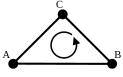
\includegraphics[width=0.4\linewidth]{ccw1}}
		\hfill
		\subbottom[\label{img:ccw_2}]{%
			\includegraphics[width=0.4\linewidth]{ccw2}}
		\hfill
	}
	\caption{Демонстрация работы предиката $ccw$}
	\label{img:ccw}
\end{figure}

Предикат $ccw$ вычисляется очень просто. Сначала необходимо посчитать детерминант $det$ матрицы \eqref{eq:det}.

\begin{equation}\label{eq:det}
det(A, B, C)= \left| \begin{array}{ccc} x_A & y_A & 1 \\ x_B & y_B & 1 \\ x_C & y_C & 1  \end{array}\right|
\end{equation}

Теперь можно определить $ccw$ через $det$ \eqref{eq:ccw}.

\begin{equation}\label{eq:ccw}
ccw(A, B, C)=det(A, B, C) > 0
\end{equation}


\subsection{Алгоритм Джарвиса} \label{subsect1_1_1}

Алгоритм Джарвиса - это один из первых придуманных алгоритмов построения выпуклой оболочки. Он был опубликован в 1972 году. %TODO ref
Этот алгоритм также называют алгоритмом заворачивания подарка, что отлично показывает суть работы алгоритма.

Пусть дано множество точек $S$. Первым делом нам надо найти такую точку $t$, чтобы было известно, что она будет лежать на выпуклой оболочке. Самый простой способ сделать это - найти левую крайнюю точку. Не теряя общности рассуждений, примем найденную точку за $t_0$. Алгоритм начинает работать при $i=0$ в точке $t_0$ и выбирает такую точку $t_{i+1}$ такую, что все остальные точки лежат правее прямой $t_i, t_{i+1}$. Также это выражается с помощью предиката \eqref{eq:ccw}:
\[
\forall p \in S \backslash \{t_i, t_{i+1}\} : ccw(t_i, t_{i+1}, p)
\]

Прямая $t_i, t_{i+1}$ на первых шагах алгоритма показана на рисунке ~\ref{img:jarvis}. Повторение этого действия пока не $t_h=p_0$ полностью построит выпуклую оболочку изначально заданного множества.

\begin{figure}[ht]
    {\centering
        \hfill
        \subbottom[\label{img:jarvis_1}]{%
            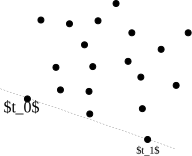
\includegraphics[width=0.4\linewidth]{jarvis1}}
        \hfill
        \subbottom[\label{img:jarvis_2}]{%
            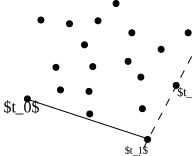
\includegraphics[width=0.4\linewidth]{jarvis2}}
        \hfill
    }
    \caption{Первые этапы работы алгоритма Джарвиса}
    \label{img:jarvis}
\end{figure}

Какова сложность алгоритма Джарвиса? Если в множестве изначально было $n$ точек, а в выпуклую оболочку попало ровно $h$ точек, то сложность алгоритма заворачивания подарка равна $O(nh)$. Доказательство этого утверждения очевидно. Так как поиск точки $t_{i+1}$ занимает проход по всему множеству точек, то это имеет сложность $O(n)$. Всего нам необходимо найти $h$ точек, так как именно столько будет находится в выпуклой оболочке.

Как видно из сложности алгоритма, он зависит не только от входных данных, но и от выходных. Это интересная особенность алгоритмов построения выпуклых оболочек, хоть и не все из них имеют сложность, зависящую от выходных данных.

\subsection{Алгоритм Грэхема} \label{subsect1_1_2}

Алгоритм Грэхема - это, наверное, самый популярный из ныне используемых алгоритмов построения выпуклых оболочек. Он очень прост в написании и при этом работает очень эффективно. Он был опубликован в 1972 году. %TODO ref

Пусть дано множество точек $S$. Первый шаг алгоритма полностью повторяет алгоритм Джарвиса - мы находим точку с самой маленькой x-координатой. Назовём эту точку $t_0$. Теперь необходимо отсортировать все остальные точки $[t_1, t_n]$ по углу относительно точки $t_0$. Это можно сделать с помощью уже знакомого предиката ccw~\eqref{eq:ccw}:
\[
A<B=ccw(t_0, A, B)
\]

Следующий этап алгоритма - это итерирование по отсортированному множеству точек. В это время все точки уже добавленные в выпуклую оболочку содержатся в стеке. Пусть сейчас добавляется точка $p$. А в стеке содержатся точки $[t_{last}, t_{last-1}, ...]$. Тогда необходимо удалить из стека такие точки, что $t_{last-1}, t_{last}, p$ образуют правый поворот. Это означает, что не выполняется $ccw(t_{last-1}, t_{last}, p)$.

На рисунке~\ref{img:graham} показан пример добавления точек при работе алгоритма Грэхема. На первом рисунке~\ref{img:graham_1} можно видеть, что добавляется точка $p_3$. Выполняется $ccw(p_1, p_2, p_3)$, поэтому точка добавляется в текущий стек. На следующем рисунке~\ref{img:graham_2} доавляется точка $p_4$, но предикат $ccw(p_2, p_3, p_4)$ не выполняется, поэтому точку $p_3$ необходимо удалить, после на рисунке~\ref{img:graham_3} видно, что это приводит к выполнению предиката $ccw(p_1, p_2, p_4)$, поэтому точка $p_4$ может быть добавлена в стек. Оставшиеся точки будут обработаны аналогичным образом, после чего мы получим готовую выпуклую оболочку состоящую из точек $p_0, p_1, p_2, p_4, p_6$.

\begin{figure}[ht]
	{\centering
		\hfill
		\subbottom[\label{img:graham_1}]{%
			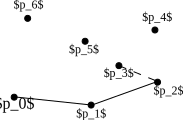
\includegraphics[width=0.3\linewidth]{graham1}}
		\hfill
		\subbottom[\label{img:graham_2}]{%
			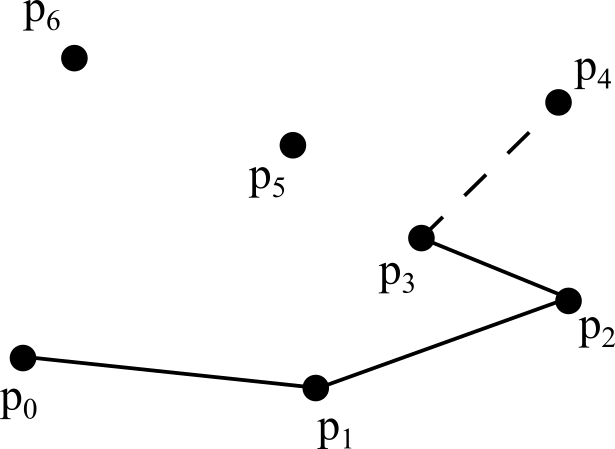
\includegraphics[width=0.3\linewidth]{graham2}}
		\hfill
		\subbottom[\label{img:graham_3}]{%
			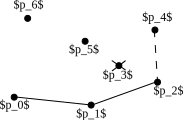
\includegraphics[width=0.3\linewidth]{graham3}}
		\hfill
	}
	\caption{Пример добавления точек при работе алгоритма Грэхема}
	\label{img:graham}
\end{figure}

Сложность этого алгоритма очень легко проанализировать. Сначала выполняется обход множества точек в поиске самой левой точки за $O(n)$. Потом необходимо отсортировать все остальные точки за $O(n \log n)$. Потом происходит обход всех точек. Заметим, что каждая точка максимум один раз добавляется в стек и один раз удаляется из него, то есть происходит $2n$ операций, что даёт сложность $O(n)$. Итоговая сложность алгоритма равна $O(n) + O(n \log n) + O(n) = O(n \log n)$.

\subsection{Разделяй и властвуй} \label{subsect1_1_3}

Принцип "Разделяй и властвуй" является очень популярным очень во многих алгоритмах в информатике. Самое знаменитое его применение - это, пожалуй, сортировка слиянием. Именно от неё во многом позаимствовал этот алгоритм для построения выпуклой оболочки множества точек.

Этот алгоритм проще всего описать с помощью рекурсивной процедуры CalcHull.

%TODO Сделать подпись не "Algorithm 1"
\begin{algorithm}
	\caption{CalcHull - функция алгоритма Разделяй и Властвуй}
	\begin{algorithmic}[1]
		\Procedure{CalcHull}{$S$}
		\If {$|S| <= 3$}
			\Return $S$
		\EndIf
		\State $leftS\gets leftOf(S)$ \Comment{Получить левую половину множества $S$}
		\State $rightS\gets rightOf(S)$ \Comment{Получить правую половину множества $S$}
		\State $leftHull\gets CalcHull(leftS)$
		\State $rightHull\gets CalcHull(rightS)$
		\State
		\Return $mergeHulls(leftHull, rightHull)$
		\EndProcedure
	\end{algorithmic}
\end{algorithm}

Сложность данного алгоритма может быть рассмотрена с помощью рекурсии, так как это и есть рекурсивная функция. Пусть изначальное множество точек состоит из $n$ элементов. Рассмотрим всё время требущееся процедуре кроме рекурсивных вызовов. Изначально нужно разделить множество точек на $leftS$ и $rightS$. Это требует $O(n)$ времени. После чего необходимо посчитать верхнюю и нижнюю касательные, и после вывести ответ. Эти действия также занимают $O(n)$ времени, что мы покажем ниже. Таким образом время может быть описано рекурсивной формулой~\ref{eq:mergeHullAnalysisBegin}.
\begin{equation}\label{eq:mergeHullAnalysisBegin}
T(n) = 3n + 2T(n/2)
\end{equation}

Как видно из ~\ref{eq:mergeHullAnalysisEnd}, сложность работы алгоритма Разделяй и Властвуй равна $O(n \log n)$.

\[
T(n) = cn \log n
\]
\[
T(n) = 3n + cn \log n/2 = 3n - cn \log 2 + cn \log n = (3 - c \log 2)n + cn \log n
\]
\begin{equation}\label{eq:mergeHullAnalysisEnd}
T(n) = 3/(\log 2)n \log n = O(n \log n)
\end{equation}

Единственное, что осталось доказать - это что можно вычислить верхнюю и нижнюю касательные за $O(n)$ время. Мы будем рассматривать только как считать нижнюю касательную, потому что верхняя может быть рассмотрена симметрично. Итак, пусть $a$ - это самая правая точка $leftHull$, а $b$ - это самая левая точка $rightHull$. Тогда пока $ab$ это не нижняя касательная ни для $leftHull$, ни для $rightHull$, необходимо попытаться продвинуть точку $a$ максимально вниз пока $ab$ не будет являтся нижней касательной для $leftHull$, а потом продвинуть точку $b$ пока $ab$ не будет являтся нижней касательной для $rightHull$. Этот процесс показан на рисунке~\ref{img:merge_1}. Финальный результат показан на втором рисунке~\ref{img:merge_2}.

\begin{figure}[ht]
	{\centering
		\hfill
		\subbottom[\label{img:merge_1}]{%
			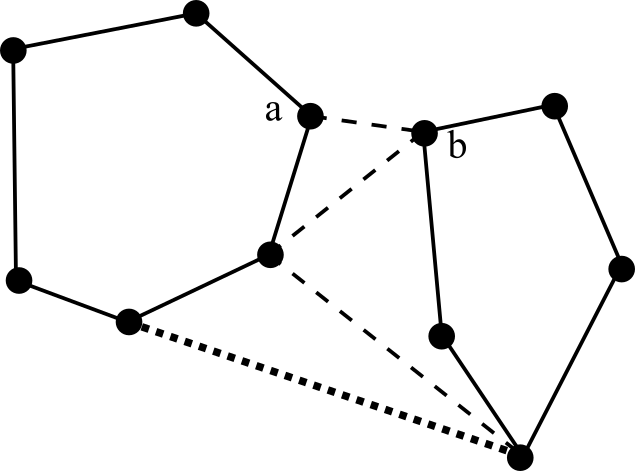
\includegraphics[width=0.4\linewidth]{merge1}}
		\hfill
		\subbottom[\label{img:merge_2}]{%
			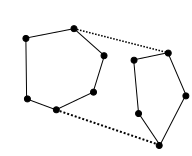
\includegraphics[width=0.4\linewidth]{merge2}}
		\hfill
	}
	\caption{Нахождение верхней и нижней касательных}
	\label{img:merge}
\end{figure}


Проверять является ли прямая нижней касательной к выпуклой оболочке очень просто. Достаточно проверить лежат ли соседние к $a, b$ точки выше этой прямой.

Очевидно, что алгоритм нахождения нижней касательной работает за $O(n)$, поэтому анализ сложности, показанный выше, верен.

\subsection{Quickhull} \label{subsect1_1_4}

Логическим продолжением алгоритма, который основан на сортировке слиянием является алгоритм основанный на быстрой сортировке. Это довольно простой и в то же время быстро работающий алгоритм. В точности как и быстрая сортировка, данный алгоритм имеет сложность $O(n \log n)$. Но в худшем случае он может работать за $O(n^2)$. Что отличет алгоритм нахождения выпуклой оболочки множества точек Quickhull и алгоритм сортировки Quicksort - это невозможность случайной перестановки до работы алгоритма, чтобы алгоритм всегда работал с сложностью $O(n \log n)$.

Самая главная идея, которая лежит в основе данного алгоритма - это убирание ненужных точек, чем раньше мы их отбросим, тем лучше. Таких точек очень много внутри выпуклой оболочки. Как правило большинство точек изначального множества окажется внутри.

Первый шаг алгоритма - это найти четыре точки у которых будут минимальные/максимальные x/y-координаты. Это даёт нам изначальное приближение к выпуклой оболочке, которую мы построим в итоге. Очевидно, что точки, который будут лежать внутри получившегося четырёхугольника можно не рассматривать, так как они будут точно лежать внутри выпуклой оболочки. Это показано на рисунке~\ref{img:quickhull_first}.

\begin{figure}[ht]
	{\centering
		\hfill
		\subbottom{%
			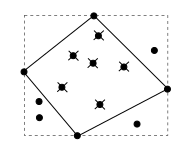
\includegraphics[width=0.4\linewidth]{quickhull1}}
		\hfill
	}
	\caption{Первый шаг алгоритма Quickhull}
	\label{img:quickhull_first}
\end{figure}

Как видно на рисунке~\ref{img:quickhull_first} после первого шага остаются точки в четырёх угловых треугольниках описанного прямоугольника. На каджом шаге алгоритма для каждого текущего ребра выпуклой оболочки мы будем рассматривать точки, которые лежат снаружи этого ребра. Все шаги алгоритма будут заключаться в том, что мы находим самую дальнюю из всех этих точек и добавляем эту точку в выпуклую оболочку. Таким образом от каждого рассмотренного ребра добавляется ещё два новых. Этот процесс показан на рисунке~\ref{img:quickhull_second} для ребра $A, B$. Как видно на~\ref{img:quickhull_second_1} мы рассматриваем некоторое множество точек на текущем шаге и находим самую дальнюю из них $C$. После чего мы добавляем эту точку к выпуклой оболочке нашего множества, что показано на рисунке~\ref{img:quickhull_second_2}.

\begin{figure}[ht]
	{\centering
		\hfill
		\subbottom[\label{img:quickhull_second_1}]{%
			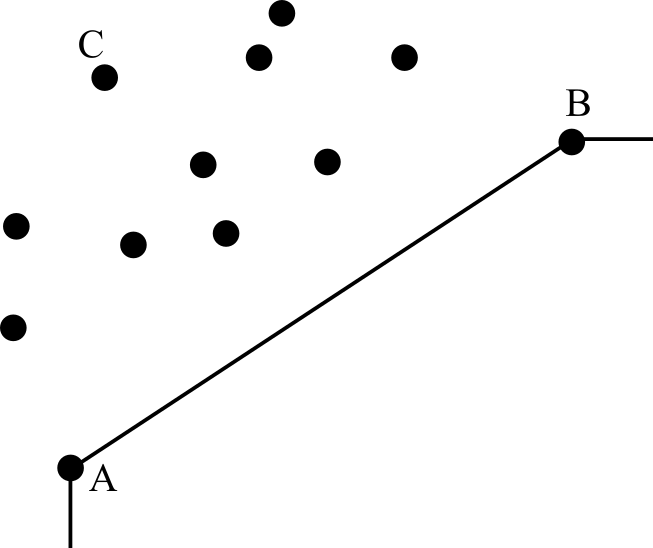
\includegraphics[width=0.4\linewidth]{quickhull2}}
		\hfill
		\subbottom[\label{img:quickhull_second_2}]{%
			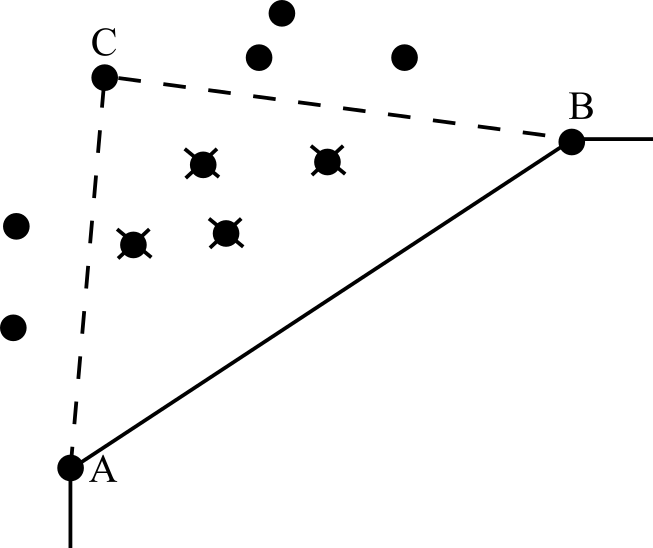
\includegraphics[width=0.4\linewidth]{quickhull3}}
		\hfill
	}
	\caption{Алгоритм Quickhull}
	\label{img:quickhull_second}
\end{figure}

Сложность алгоритма Quickhull, в точности как и quicksort, зависит от того, насколько ровно будут разбиваться точки на 2 части при добавлении самой дальней из них. Пусть $T(n)$ - это время работы алгоритма в зависимости от количества точек поступивших на вход $n$. За один проход по точкам мы можем определить точку, которая будет разбивать наше множества на 2, которые должны быть рассмотрены далее. Пусть $n_1, n_2$ - это количества точек в подмножествах после разбиения. Очевидно, что $n_1+n_2<=n$. Таким образом время может быть описано рекурсивной формулой~\ref{eq:quickHullAnalysisBegin}.

\begin{equation}\label{eq:quickHullAnalysisBegin}
T(n) = n + T(n_1) + T(n_2)
\end{equation}

Чтобы решить эту формулу, необходимо выбрать некоторые значения для $n_1$ и $n_2$. Если предположить, что точки более или менее ровно разбиваются, что описывается формулой~\ref{eq:quickHullAnalysisConstant}, то можно доказать, что время работы алгоритма будет $O(n \log n)$. Если же разбиения не ровные, то время работы алгоритма легко может стать $O(n^2)$.

%TODO: Добавить ссылку на источник + возможно, описать самому вывод функции сложности

\begin{equation}\label{eq:quickHullAnalysisConstant}
\exists  a < 1 : max(n_1, n_2) <= a * n
\end{equation}

Этот алгоритм может быть очень хорош на некотором наборе точек, и чаще всего он отлично работает. Причём как видно из описания алгоритма он отбрасывает очень много ненужных точек на каждом шаге, что делает его замечательным для использования, если бы не плохое время при специально подобранном наборе точек. Поэтому на практике всё равно предпочитают алгоритм Грэхема.

\subsection{Инкрементальный алгоритм} \label{subsect1_1_5}

% TODO: Добавить ссылку на источник описания алгоритма

Инкрементальный алгоритм - это алгоритм, на который мы будем опираться больше всего при построении нашего собственного. Он использует 2 бинарных дерева поиска для построения выпуклой оболочки. Основная идея алгоритма в том, что мы будем добавлять точки в произвольном порядке и для текущих добавленных точек будет поддерживаться текущая выпуклая оболочка. Получается, что необходима такая структура данных, которая должна определять точка находиться внутри или снаружи выпуклой оболочки. После чего если точка находится снаружи, то необходимо её добавить к текущей выпуклой оболочке с учётом того, что необходимо удалить точки, которые уже не принадлежат выпуклой оболочке.

Эффективная структура данных для такого алгоритма - это бинарное дерево поиска. Мы будем хранить текущую выпуклую оболочку в двух деревьях. Верхнее $T_H$ и нижнее $T_L$ деревья будут представлять верхнюю и нижнюю части выпуклой оболочки. То есть, чтобы в конце получить результат необходимо слить эти две цепочки в один цикл. Эти деревья показаны на рисунке \ref{img:incremental_trees}.

Существует 2 типа вершин, в таких деревьях:
\begin{enumerate}
	\item Внутренние вершины деревьев представляют собой пары $(v_x, v)$, где $v$ - это точка, которая сейчас находится на выпуклой оболочке, а $v_x$ - координата $x$ этой точки. Таким образом точка отсортированы по координате $x$. Они показаны кружками на рисунке \ref{img:incremental_trees}.
	\item Внешние вершины представляют собой либо ребро выпуклой оболочки, либо пустую полуплоскость в случае крайней левой и крайней правой вершин. Они показаны квадратами на рисунке \ref{img:incremental_trees}.
\end{enumerate}

\begin{figure}[ht] 
	\centering
	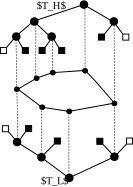
\includegraphics [scale=0.7]{incremental1}
	\caption{Структура данных для инкрементального алгоритма}
	\label{img:incremental_trees}
\end{figure}

Опишем процесс поиска вершина снаружи или внутри в такой структуре. Пусть ищется точка $q$. Тогда необходимо в деревьях $T_H$ и $T_L$ найти ребро или вершину, которая находится в точке $q_x$. Назовём найденные точки и ребра $v_L, e_L, v_H, e_H$ для нижнего и верхнего дерева соответственно. Пример получившегося результата показан на рисунке \ref{img:incremental_locate}.

Рассмотрим 4 случая:
\begin{enumerate}
	\item Если нет таких ребёр или вершин, тогда эта точка находится снаружи выпуклой оболочки.
	\item Если точка находиться в вершине $v_L, v_H$ или на ребре $e_L, e_H$, то $q$ лежит на выпуклой оболочке.
	\item Если $q$ ниже $e_H (v_H)$ и выше $e_L (v_L)$, то $q$ лежит внутри выпуклой оболочки.
	\item Иначе $q$ лежит снаружи выпуклой оболочки.
\end{enumerate}

\begin{figure}[ht] 
	\centering
	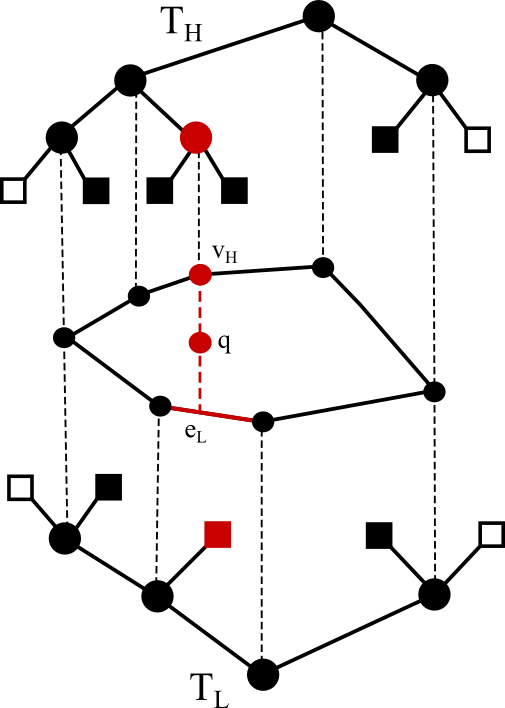
\includegraphics [scale=0.7]{incremental2}
	\caption{Нахождение вершин, соответствующих точке $q$}
	\label{img:incremental_locate}
\end{figure}

Как видно, для того, чтобы определить точка лежит или снаружи необходимо сделать довольно много действий. Но как, например, определить точка $q$ находится выше ребра $a, b$  или нет? В этом снова помогает предикат $ccw$, описанный в формуле \ref{eq:ccw}. Точка находится выше если $ccw(a, b, q)$. Это показано на рисунке \ref{img:incremental_ccw}.

\begin{figure}[ht] 
	\centering
	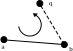
\includegraphics {incremental3}
	\caption{Определение положения точки с помощью предиката $ccw$}
	\label{img:incremental_ccw}
\end{figure}

После определения точка $q$ лежит внутри или снаружи выпуклой оболочки, необходимо добавить эту точку. Куда добавлять точку $q$ определяется на основе её положения. Существует 4 случая:
\begin{enumerate}
	\item Если точка лежит внутри или на выпуклой оболочке, то добавлять $q$ не нужно.
	\item Если точка снаружи и сверху, то необходимо добавить её в дерево $T_H$.
	\item Если точка снаружи и снизу, то необходимо добавить её в дерево $T_L$.
	\item Если точка снаружи и справа или слева, то необходимо добавить её как в $T_L$, так и в $T_H$.
\end{enumerate}

Все возможные случаи показаны на рисунке %TODO: add picture

%TODO: add picture here

Последнее, что необходимо определить в этом алгоритме - это как правильно добавлять точку в дерево. Опишем это с помощью псевдокода:

%TODO: add code here

%TODO: рассказать про сложность алгоритма

\subsection{Алгоритм Чана} \label{subsect1_1_6}

\section{Анализ текущего состояния алгоритмов и выявление проблемы} \label{sect1_2}

\section{Требования, предъявляемые к разрабатываемому алгоритму} \label{sect1_3}







